\begin{frame}
    \frametitle{前情回顾}
    {\Bullet} 一个自由度为$n$的系统由$n$对正则变量($q_1, q_2, \cdots, q_n, p_1, p_2, \cdots, p_n$)描述, 每对正则共轭变量($q_i, p_i$)符合正则方程:
    \[ \frac{\mathrm{d} q_i }{\mathrm{d} t}  = \frac{\partial H }{\partial p_i}, \quad \frac{\mathrm{d} p_i }{\mathrm{d} t}  = - \frac{\partial H }{\partial q_i}\]
    所有物理量都可用正则变量表示,比如哈密顿\[H(q_1, q_2, \cdots, q_n, p_1, p_2, \cdots, p_n) \] 
    {\Bullet} 正则量子化: 
    \begin{itemize}
        \item 写出经典哈密顿;
        \item 哈密顿正则化;
        \item 正则变量算符化; 哈密顿算符化(其他物理量也可算符化);
        \item 把哈密顿算符代入薛定谔方程求解.
    \end{itemize}     
\end{frame}

%%%%%%%%%%%%%%%%%%%%%%%%%%%%%%%%%%%%%%%%%%%%%%%%%%%%%%%%%%%%%
\begin{frame} [plain]
    \frametitle{}
    \Background[1] 
    \begin{center}
    {\huge 第4-5讲:光场量子化}
    \end{center}  
    \addtocounter{framenumber}{-1}   
\end{frame}
%%%%%%%%%%%%%%%%%%%%%%%%%%%%%%%%%%%%%%%%%%%%%%%%%%%%%%%%%%%% 


\section{1. 单模光场的量子化}

\begin{frame}
      \frametitle{电磁场的哈密顿}
    考虑空腔中的线性极化电磁波,如图 
    \begin{center}
     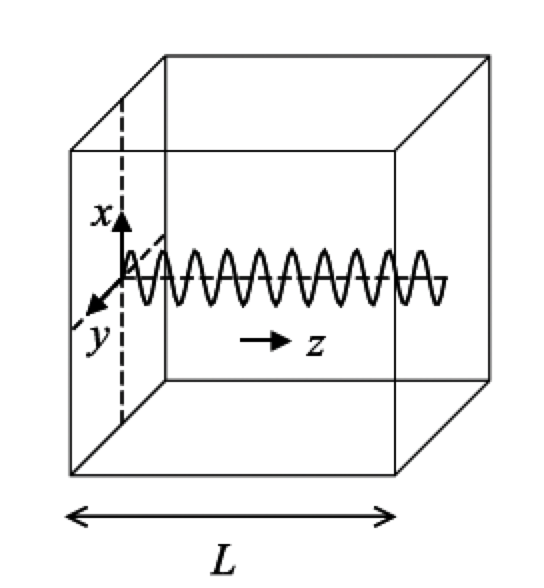
\includegraphics[width=0.45\textwidth]{figs/2022-04-27-12-37-33.png}
    \end{center}     
\end{frame}

\begin{frame}
      \frametitle{}
    经典解:
      \begin{enumerate}
        \IItem 电场:$\displaystyle E_{x}(z,t) = \sum\limits_{l=1}^{\infty } E_{0}  \sin \omega_l t \sin k_l z= \sum\limits_{l=1}^{\infty } a_l q_l (t) \sin (k_l z)$
        \IItem 磁场: $\displaystyle H_{y}(z,t) = \sum\limits_{l=1}^{\infty } H_{0}  \cos \omega_l t \cos k_l z = \sum\limits_{l=1}^{\infty } a_l \frac{\varepsilon_0}{k_l}q_l ' (t) \cos (k_l z)$  
    \end{enumerate}	  
    电磁场的能量密度: 
    \[ \omega = \frac{1}{2} (\varepsilon_0 E^2 _x + \mu_0 H^2 _y) \]
    经典哈密顿:
    \[ H = \frac{1}{2} \int_V (\varepsilon_0 E^2 _x + \mu_0 H^2 _y) dV \] 
\end{frame}

\begin{frame}
      \frametitle{}
    代入电磁场经典解, 利用腔模正交性, 得:
    \[ \begin{aligned}
        H &= \frac{1}{2} \int_V (\mu_0 \mathbf{H}^2 + \varepsilon_0 \mathbf{E}^2) dV \\ 
        &= \sum_l  \frac{1}{2}(p_l ^2 + \omega_l ^2 q_l ^2 ) \\ 
        &= \sum_l H_l  
     \end{aligned} 
    \] 
    电磁场总哈密顿是单模哈密顿的线性叠加.
\end{frame}

\begin{frame}
      \frametitle{单模量子化}
      单模哈密顿:
      \[ H_l  =  \frac{1}{2}(p_l ^2 + \omega_l ^2 q_l ^2 ) \]
      写出密顿运动方程
    \[ \begin{aligned}
        \frac{\mathrm{d}p_l}{\mathrm{d}t} &= - \frac{\partial H_l}{\partial q_l} = - \omega ^2 _l q_l \\ 
        \frac{\mathrm{d}q_l}{\mathrm{d}t} &= \frac{\partial H_l}{\partial p_l} =p_l
        \end{aligned} 
    \] 
    说明 $ p_l $ 和$q_l$ 是一对正则量.  可进行正则量子化!
\end{frame}

\begin{frame}    
    量子化条件
    \[  [\hat{q}_l,\hat{p}_l]=i\hbar \] 
    写在一起:
    \[ \hat{H}_l  =  \frac{1}{2}(\hat{p}_l ^2 + \omega_l ^2 \hat{q}_l ^2 )  \qquad \text{with} \quad [\hat{q_l},\hat{p_l}] =i\hbar\] 
    代入薛定谔方程,既可求得场的波函数! \\ {\vspace*{1em}}
  \end{frame}
  
  \begin{frame} 
  \frametitle{求解单模光场}
    单模哈密顿
    \[ \hat{H}_l  =  \frac{1}{2}(\hat{p}_l ^2 + \omega_l ^2 \hat{q}_l ^2 )  \qquad \text{with} \quad [\hat{q_l},\hat{p_l}] =i\hbar\] 
    谐振子哈密顿
    \begin{equation*}
        \hat{H} = \frac{\hat{p}^2 }{2m} + \dfrac{1}{2} m \omega ^2 \hat{x}^2   \qquad \text{with} \quad [\hat{x},\hat{p}]=i\hbar 
    \end{equation*}	
    比较: 如果令谐振子质量$m =1$, 则形式完全相同.  \\ 
    单模光场可视为单位质量的谐振子. 并称$\hat{q_l},\hat{p_l}$为电场和磁场算符\\ {\vspace*{1.3em}}
    * 机械振子通过动-势能的相互转换形成振荡, 光场通过电场能和磁场能的相互转换形成振荡!
\end{frame}

\begin{frame}   
  ~{\Bullet}具体求解与谐振子相同, 令:
    \[ \hat{Q}_l = \sqrt{\frac{\omega}{\hbar}}\hat{q_l}, \qquad \hat{P}_l = \sqrt{\frac{1}{\hbar \omega}} \hat{p_l} \]
    有:
    \[  \hat{H}_l= \frac{\hbar \omega }{2} (\hat{Q}^2 _l + \hat{P}^2 _l) \qquad \text{with} \quad [\hat{Q}_l,\hat{P}_l]=i \]
    令:
    \[ \hat{a}_l= \frac{1 }{\sqrt{2}} (\hat{Q} _l+ i\hat{P}_l ), \qquad \hat{a}^\dagger _l = \frac{1 }{\sqrt{2}} (\hat{Q}_l - i\hat{P}_l ) \]
    有
    \[
        \hat{a}_l = \frac{1}{\sqrt{2\hbar \omega_l}} (\omega_l\hat{q}_l+i \hat{p}_l)  , \qquad
        \hat{a}_l ^\dagger = \frac{1}{\sqrt{2\hbar \omega_l}} (\omega_l\hat{q}_l-i \hat{p}_l)  
    \]  
    可得产生湮灭形式:
    \[  \hat{H}_l= \hbar \omega \left(\hat{a}^\dagger _l \hat{a} _l + \frac{1 }{2}\right) \qquad \text{with} \quad [\hat{a}_l,\hat{a}^\dagger _l]=1 \]
\end{frame}

\begin{frame} 
\frametitle{}
~\\
    量子谐振子中取质量 $m=1$, 即得单模光场($\omega_l$)解 \\  \vspace*{1.3em}
    能量本征值
    \[ E_n=(n+\dfrac{1}{2})\hbar \omega_l \]
    能量本征态
    \[ \rs{n} \]
    位置表象的能量本征态
    \[ \lr{x}{n} = \frac{1}{\sqrt{n!2^n}} (\frac{\alpha}{\pi})^{\frac{1}{4}} e^{- \frac{1 }{2 } \xi^2} H_n(\xi) \]
    式中
    \[ \xi = \alpha x, \qquad \alpha =\sqrt{\frac{m \omega }{\hbar}} = \sqrt{\frac{\omega }{\hbar}}  \]
    解毕!
\end{frame}


\begin{frame}
  \frametitle{电磁场的其他物理量}
  ~\\
  根据
  \[
    \hat{a}_l = \frac{1}{\sqrt{2\hbar \omega_l}} (\omega_l\hat{q}_l+i \hat{p}_l)  , \qquad
    \hat{a}_l ^\dagger = \frac{1}{\sqrt{2\hbar \omega_l}} (\omega_l\hat{q}_l-i \hat{p}_l)  
    \]  
  反向求得: 
  \[ \begin{aligned}
     \hat{q}_l &= \sqrt{\frac{\hbar}{ 2\omega_l}} (\hat{a}_l+ \hat{a}_l ^\dagger) \\ 
     \hat{p}_l &= -i\sqrt{\frac{\hbar\omega_l}{2 }} (\hat{a}_l- \hat{a}_l ^\dagger)  
  \end{aligned} \] 
若光场的某物理量F的经典表示为:$F(q_l, p_l)$, 则其量子力学算符为: $F(\hat{q}_l, \hat{p}_l)$, 其产生湮灭算符形式也可求得. \\ {\vspace*{1.3em}}

即: 电磁场的所有经典物理量都可经由产生湮灭算求得!     
\end{frame}

\begin{frame}
    \frametitle{}
    \例 [1.求单模腔场电磁场分量的算符形式] {}
    \解 ~经典单模腔场解: 
    \[ \begin{aligned}
      E_{l}(z,t) &= a_l q_l (t) \sin (k_l z)\\
      H_{l}(z,t) &= b_l p_l (t) \cos (k_l z)
    \end{aligned}\] 
    算符:
    \[ \begin{aligned}
      \hat{E}_{x,l}(z,t) &= a_l \hat{q}_l (t) \sin (k_l z)\\
      \hat{H}_{y,l}(z,t) &= b_l \hat{p}_l (t) \cos (k_l z)
    \end{aligned}\] 
    代入
      \[ \begin{aligned}
        \hat{q}_l = \sqrt{\frac{\hbar}{ 2\omega_l}} (\hat{a}_l+ \hat{a}_l ^\dagger) , \qquad  
        \hat{p}_l = -i\sqrt{\frac{\hbar\omega_l}{2 }} (\hat{a}_l- \hat{a}_l ^\dagger)  
     \end{aligned} \] 
\end{frame}

\begin{frame} 
\frametitle{}
    产生湮灭算符描述的电场算符
    \[ 
      \hat{\mathbf{E}}_{x,l}( z,t) = E^0 _l \left(\hat{a}_l(t)+ \hat{a}_l ^\dagger(t) \right) \sin (k_l z)
      \] 
    式中 \[ E^0 _l = \sqrt{\frac{\hbar \omega_l }{\varepsilon_0 V}}\]
    三维形式
    \[ \hat{\mathbf{E}}_l(\mathbf{r},t) = E^0 _l \left(\hat{a}_l(t)+ \hat{a}_l ^\dagger(t) \right) \mathbf{E}_l(\mathbf{r}) \]
\end{frame}

\begin{frame}
  \frametitle{}
  \例 [2.试证明电场算符与占据数算符不对易] {\[ [\hat{n}, \hat{E}_x] = E_0 \sin{kz}(\hat{a}^{\dagger}-\hat{a})\]}
  \解 ~考虑单模场:
  \[ \begin{aligned}
    [\hat{n}, \hat{E}_x] &= \left[\hat{a}^{\dagger}_l \hat{a}_l, E^0 _l \left(\hat{a}_l+ \hat{a}_l ^\dagger \right) \sin (k_l z)\right] \\
    &= E^0 _l\sin (k_l z)\left[\hat{a}^{\dagger}_l \hat{a}_l,  \left(\hat{a}_l+ \hat{a}_l ^\dagger \right)\right]\\ 
    &= E^0 _l\sin (k_l z)\hat{a}^{\dagger}_l\left[ \hat{a}_l,  \left(\hat{a}_l+ \hat{a}_l ^\dagger \right)\right] + E^0 _l\sin (k_l z)\left[\hat{a}^{\dagger}_l ,  \left(\hat{a}_l+ \hat{a}_l ^\dagger \right)\right]\hat{a}_l\\
    &=  E^0 _l\sin (k_l z)\hat{a}^{\dagger}_l- E^0 _l\sin (k_l z)\hat{a}_l \\ 
    &= E_0 \sin{kz}(\hat{a}^{\dagger}-\hat{a})
  \end{aligned}\] 
  证毕!\\
  说明:电场越确定, 则光场的光子数越不确定,也即场强与相位不能同时确定。
\end{frame}

\section{2. 单模光场的量子涨落}

\begin{frame}
      \frametitle{}
    \例[3.试证明$Fock$ 态下电磁场的电场强度平均值为零]{}
    \证~
    设电磁场处于$Fock$ 态 $\rs{n}$, 取三维腔模进行计算
    \[ 
      \begin{aligned}
        \lcr{n}{\mathbf{E}(\mathbf{r,t})}{n} &= \lcr{n}{E^0  (\hat{a}+ \hat{a} ^\dagger)\mathbf{E}(\mathbf{r})}{n}   \\ 
        &= E^0 \mathbf{E}( \mathbf{r})\lcr{n}{\hat{a} }{n} + E^0 \mathbf{E}( \mathbf{r})\lcr{n}{\hat{a}^\dagger }{n}  \\ 
        &= 0+0 \\ 
        &=0 
      \end{aligned}
      \]   
      ~\\
      * 相位随机性导致测量平均值为零!  (证明见后)\\
      Fock态表象一般用于处理小粒子数的情况.  \\      
\end{frame}

\begin{frame}
    \frametitle{}
    \例[4.考虑一维单模驻波场, 求电场和磁场强度的量子涨落]{}
    \解~一维单模驻波场的电场和磁场算符为  
    \[ \begin{aligned}
      E_x(z,t)
      &= E_0  (a(t)+a^\dagger(t) )\sin (kz) \\
   \end{aligned} \]
   设光场处于$Fock$态$\rs{n}$, 有:
   \[ \lcr{n}{E_x(z,t)}{n} = \lcr{n}{H_y(z,t)}{n} =0\]
  \end{frame}

  \begin{frame}
   \[ \begin{aligned}
     \lcr{n}{E^2_x}{n} &= \lcr{n}{E^2_0 \sin^2 (kz) (a^\dagger(t)-a(t))^2}{n} \\
     &= E^2_0 \sin^2 (kz) \lcr{n}{2a^\dagger a+1}{n} \\ 
     &= 2 E^2_0 \sin^2 (kz) \lcr{n}{n+\frac{1}{2}}{n} \\ 
     &= 2 (n+\frac{1}{2})E^2_0 \sin^2 (kz)  
  \end{aligned} \]
  量子涨落: 
  \[
 \begin{aligned}
        \Delta E_x &= \sqrt{\langle E^2_x\rangle - \langle E_x\rangle ^2} \\
        &= \sqrt{2} \sqrt{n+\frac{1}{2}} E_0 \left|\sin kz \right| 
 \end{aligned} \]
 即使没有激发(n=0),依然存在真空涨落$ E_0 \left|\sin kz \right|  $  
\end{frame}

%%%%%%%%%%%%%%%%%%%%%%%%%%%%%%%%%%%%%%%%%%%%%%%%%%%%%%%%%%%%%%%%%%%
\begin{frame}
  \frametitle{课堂作业}
   \begin{block}{试证明如下重要结论}
   \[
  \begin{aligned}
   \lcr{n}{\hat{a} ^\dagger\hat{a} ^\dagger}{n} & = 0   \\     
   \lcr{n}{\hat{a} \hat{a} }{n} & =0   \\  
   \lcr{n}{\hat{a} ^\dagger\hat{a} }{n} & = n   \\   
   \lcr{n}{\hat{a} \hat{a} ^\dagger}{n} & = n+1   \\    
  \end{aligned}
  \]
   \end{block}
\end{frame}
%%%%%%%%%%%%%%%%%%%%%%%%%%%%%%%%%%%%%%%%%%%%%%%%%%%%%%%%%%%%%%%%%%%

\section{3. 光场随时间的演化}

\begin{frame}
 \frametitle{}
 {\Bullet}海森堡方程描述算符随时间的演化规律:
 \[ i\hbar\frac{\mathrm{d}F}{\mathrm{d}t} = [F,H] \]
 把$F= a $ 和光场哈密顿代入上式
 \[ \begin{aligned}
   \frac{\mathrm{d}a}{\mathrm{d}t} & =  \frac{1}{i \hbar} \left[a, \hbar \omega \left(\hat{a}^\dagger \hat{a} + \frac{1 }{2}\right)\right] \\
   &= i \omega (a^{\dagger} a a - a a^{\dagger}a)\\
   &= i \omega [a , a^{\dagger}] a \\ 
   &= - i \omega a
 \end{aligned}\] 
解得:
 \[ a(t)=a(0) e^{-i \omega t} = a e^{-i \omega t} \]  
同理,  
 \[ a ^\dagger(t)=a ^\dagger(0) e^{i \omega t} = a ^\dagger e^{i \omega t}\]  
\end{frame}

\begin{frame}
 \frametitle{}
 场算符随时间的演化:
\[ q_{l}(t)=\sqrt{\frac{\hbar}{2 \omega_{l}}}\left(a_{l} e^{-i \omega_{l} t}+a_{l}^{\dagger} e^{i \omega_{l} t}\right) \]
\[ p_{l}(t)=- i\sqrt{\frac{ \hbar \omega_{l}}{2}}\left(a_{l} e^{-i \omega_{l} t}-a_{l}^{\dagger} e^{i \omega_{l} t}\right) \]   
\end{frame}

\begin{frame}
 \frametitle{}
  场强随时间的演化 
  \[ 
    \begin{aligned}
      &E_{x}(z, t)=\sum_{l} \mathcal{E}_{l}^{(s)}\left(a_{l} e^{-i \omega t}+a_{l}^{\dagger} e^{i \omega t}\right) \sin \left(k_{l} z\right)  \\ 
      &B_{y}(z, t)=-i \sum_{l} \mathcal{B}_{l}^{(s)}\left(a_{l} e^{-i \omega t}-a_{l}^{\dagger} e^{i \omega t}\right) \cos \left(k_{l} z\right)  \\   
    \end{aligned} 
  \]
式中 $\mathcal{E}_{l}^{(s)}=\sqrt{\frac{\hbar \omega_{l}}{\varepsilon_{0} V}}, \quad
\mathcal{B}_{l}^{(s)}=\frac{\mu_0}{k_l}\sqrt{\frac{\varepsilon_{0}\hbar \omega_{l} ^3}{V}}$
\end{frame}

\section{4. 量子化相图}

\begin{frame}
  \frametitle{经典相图}
  考虑空腔中的一个线性极化的电磁波,如图
    \begin{center}
       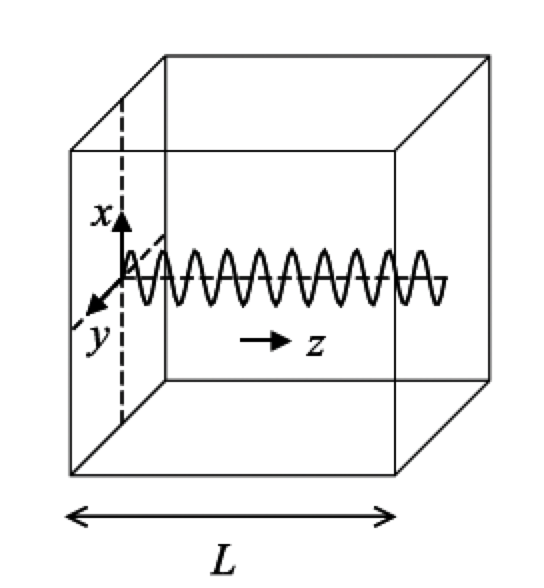
\includegraphics[width=0.24\textwidth]{figs/2022-04-27-12-37-33.png}
    \end{center}
   场分量如下:  
   \[ \begin{cases}
    E_{x}(z, t)=E_{0} \sin \omega t\sin k z  \\ 
    B_{y}(z, t)=B_{0} \cos \omega t \cos k z,  \quad \text{with} \quad B_{0} = E_{0} /c 
   \end{cases} \]
 \end{frame}
 
%\begin{frame}
% \frametitle{}
% 电磁场的能量密度为:
% \[ H=\frac{1}{2}\left(\epsilon_{0} {E}^{2}+\frac{1}{\mu_{0}} B^{2}\right) \]
% 电场能 (设模面积为A): 
% \[ \begin{aligned}
%  E_{\text {electric }} &=\frac{1}{2} \epsilon_{0} A \int_{0}^{L} {E}_{0}^{2} \sin ^{2} k z \sin ^{2} \omega t \mathrm{~d} z \\
%  &=\frac{1}{4} \epsilon_{0} A {E}_{0}^{2} \sin ^{2} \omega t \int_{0}^{L}(1-\cos 2 k z) \mathrm{d} z \\
%  &=\frac{1}{4} \epsilon_{0} V {E}_{0}^{2} \sin ^{2} \omega t
%  \end{aligned}
%    \]       
%\end{frame}
%
%\begin{frame}
% \frametitle{}
% 磁场能 :  
% \[\begin{aligned}
%  E_{\text {magnetic }} &=\frac{1}{2 \mu_{0}} A \int_{0}^{L} B_{0}^{2} \cos ^{2} k z \cos ^{2} \omega t \mathrm{~d} z \\
%  &=\frac{1}{4 \mu_{0}} A B_{0}^{2} \cos ^{2} \omega t \int_{0}^{L}(1+\cos 2 k z) \mathrm{d} z \\
%  &=\frac{1}{4 \mu_{0}} V B_{0}^{2} \cos ^{2} \omega t
%  \end{aligned} \] 
%总能量 :
%\[ H=\frac{V}{4}\left(\epsilon_{0} \mathcal{E}_{0}^{2} \sin ^{2} \omega t+\frac{B_{0}^{2}}{\mu_{0}} \cos ^{2} \omega t\right)
%   \]
%\end{frame}
%
%begin{frame}
% \frametitle{}
% 令: \[ q(t)=\left(\frac{\epsilon_{0} V}{2 \omega^{2}}\right)^{1 / 2} \mathcal{E}_{0} \sin \omega t \]
% \[ p(t)=\left(\frac{V}{2 \mu_{0}}\right)^{1 / 2} B_{0} \cos \omega t \equiv\left(\frac{\epsilon_{0} V}{2}\right)^{1 / 2} \mathcal{E}_{0} \cos \omega t \]
% 代回, 得总能:
%     \[ H=\frac{1}{2}\left(p^{2}+\omega^{2} q^{2}\right) \]
% 说明电磁场的振荡是电场能与磁场能之间的转换
%end{frame}

\begin{frame}
 \frametitle{}
 初始条件决定一个初始相位 $ \varphi$ \\ 
  {\Bullet}复函表示:  \[
    \begin{aligned}
         E_{x}(z, t) &= E_{0} \sin (\omega t+\varphi) \sin k z \\
         &=E_{0} (z,t) e^ {i\varphi}  \\
         &=  E_{0}(z,t) \cos\varphi  + i E_{0}(z,t) \sin\varphi \\ 
         &= E_1 (z,t) + i E_2 (z,t)
    \end{aligned}
    \]
  其中 $E_1(z,t), E_2(z,t) $是电场的实部和虚部 \\   
\end{frame}

\begin{frame}
   \begin{center}
      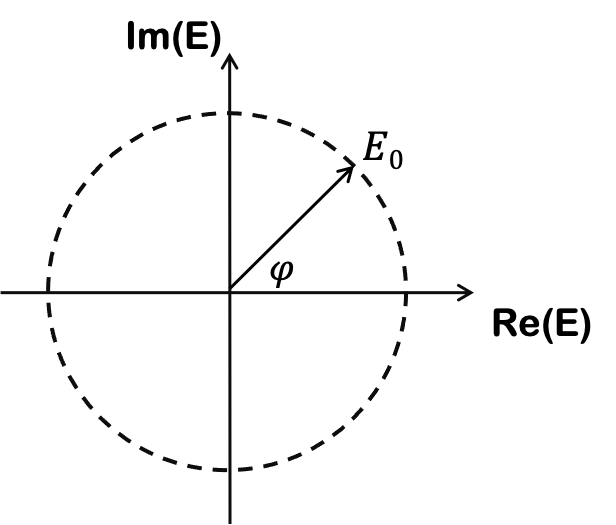
\includegraphics[width=0.4\textwidth]{figs/2.png}
   \end{center}
 \[ \begin{cases}
  Re(E)= E_{0}(z,t) \cos\varphi\\ 
  Im(E)= E_{0}(z,t) \sin\varphi\\ 
 \end{cases} \]
 电磁场的大小和相位角都是确定的.  
\end{frame}

\begin{frame}
  \frametitle{}
  定义电场的正交分量(field quadratures)
  \[ \begin{cases}
    X_{1}(t) = \sqrt{\frac{\omega}{2\hbar}}q(t)= \sqrt{\frac{\varepsilon_{0} V}{4 \hbar \omega}} {E}_{0} \sin \omega t\\ 
    X_{2}(t) = \sqrt{\frac{1}{2\hbar \omega}}p(t)= \sqrt{\frac{\varepsilon_{0} V}{4 \hbar \omega}} {E}_{0} \cos \omega t\\ 
   \end{cases} \]
   代入
   \[
  \begin{aligned}
       E_{x}(z, t) &=E_{0} \sin k z \sin (\omega t + \varphi) \\
       &=  E_{0} \sin k z (\cos\varphi \sin\omega t + \sin\varphi \cos\omega t) \\ 
       &= \sqrt{\frac{4 \hbar \omega}{\varepsilon_{0} V}} \sin k z\left(\cos \varphi X_{1}(t)+\sin \varphi X_{2}(t)\right) \\ 
       &=  X_{1}(z,t)+ i X_{2}(z,t)
  \end{aligned}
  \]
\end{frame}

\begin{frame}
  \begin{center}
     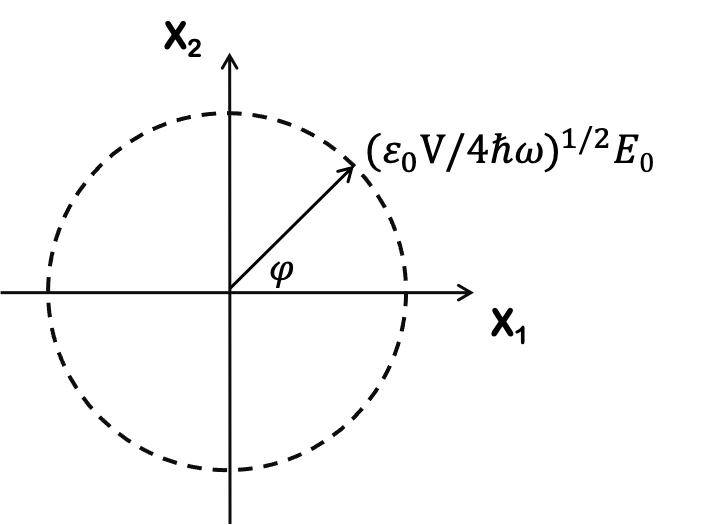
\includegraphics[width=0.5\textwidth]{figs/3.png}
  \end{center}
\end{frame}


\begin{frame}
  \frametitle{量子化相图}
  场正交分量可量子化:
  \[ \begin{cases}
    \hat{X}_{1}(t) = \sqrt{\frac{\omega_l}{2\hbar}}\hat{q}(t)=\frac{1}{2}\left(a+a^{^{\dagger}}\right)\\ 
    \hat{X}_{2}(t) = \sqrt{\frac{1}{2\hbar \omega_l}}\hat{p}(t)= \frac{1}{2 i}\left(a-a^{^{\dagger}}\right)\\ 
   \end{cases} \]
  \[ \text{with} \, [X_1, X_2] =\frac{i}{2} \]
  计算不确定度:
  \[ \Delta X_1 \Delta X_2  = \frac{1}{2\hbar}  \Delta q \Delta p \geq \frac{1}{2\hbar} \frac{\hbar}{2}=\frac{1}{4}  \]
\end{frame}

\begin{frame}
    \frametitle{} 
    \begin{center}
       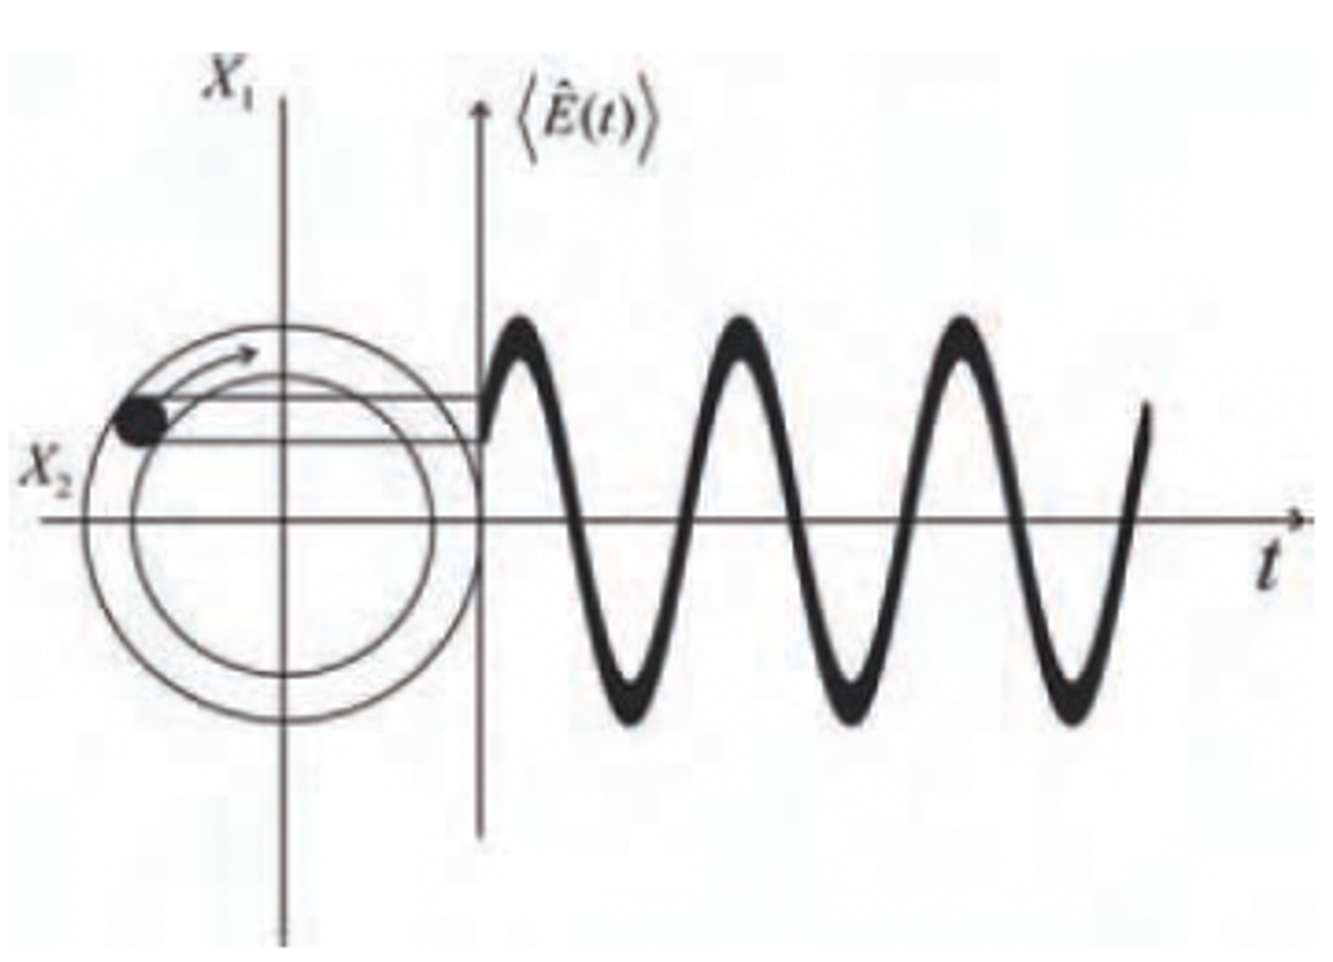
\includegraphics[width=0.55\textwidth]{figs/34.png}
    \end{center}
    \[ \Delta X_1 \Delta X_2  \geq  \frac{1}{4}  \]
    电磁场的大小和相位角都有一定的不确定性. 黑色区描述不可区分的简并态. 
\end{frame}

\begin{frame}
  \frametitle{}
  \例[5.试证明真空态是最小不确定度乘积态]{
   \[ \Delta X_1 \Delta X_2 =\dfrac{1}{4} \] 
  }
  \解~不确定度计算公式\[ \Delta x  = \sqrt{ \overline{x^2}- \overline{x}^2}\] 
\[ 
\begin{aligned}
  \overline{ X_1}  &= \lcr{n}{\frac{1}{2}\left(a+a^{\dagger}\right)}{n} \\ 
        &= 0 \\
  \overline{ X_2 } &= \lcr{n}{\frac{1}{2i}\left(a-a^{\dagger}\right)}{n} \\ 
        &= 0 
\end{aligned}\]
\end{frame}

\begin{frame}
  \frametitle{}
\[ 
\begin{aligned}
  \overline{X_1 ^2} &= \lcr{n}{\frac{1}{4}\left(a+a^{\dagger}\right)^2}{n} \\
        &= \frac{1}{4} \lcr{n}{\left(aa+a^{\dagger}a^{\dagger}+aa^{\dagger}+ a^{\dagger}a\right)}{n} \\
        &= \frac{1}{4} (2n+1)
\end{aligned}\]
\[
\begin{aligned}
  \overline{X_2 ^2} &= \lcr{n}{-\frac{1}{4}\left(a-a^{\dagger}\right)^2}{n} \\
  &= -\frac{1}{4} \lcr{n}{\left(aa+a^{\dagger}a^{\dagger}-aa^{\dagger}- a^{\dagger}a\right)}{n} \\
  &= \frac{1}{4} (2n+1)
\end{aligned}\]
\[ \Delta X_1 = \Delta X_2  =  \sqrt{ \overline{X^2}- \overline{X}^2} =\frac{1}{2}\sqrt{2n+1}\geq \frac{1}{2}\] 
\end{frame}

\begin{frame}
 \frametitle{}
  对于真空态
 \[ \Delta X_1 = \Delta X_2  = \frac{1}{2}\]
 即:
 \[ \Delta X_1 \Delta X_2  = \frac{1}{4}\]    
 证毕!\\ 
\end{frame}

\begin{frame}
 \frametitle{真空态相图}
真空态的经典电场能$E_0=0$, 电场矢量大小为零, 处于原点. 是相位完全不确定的态. 
      \begin{center}
         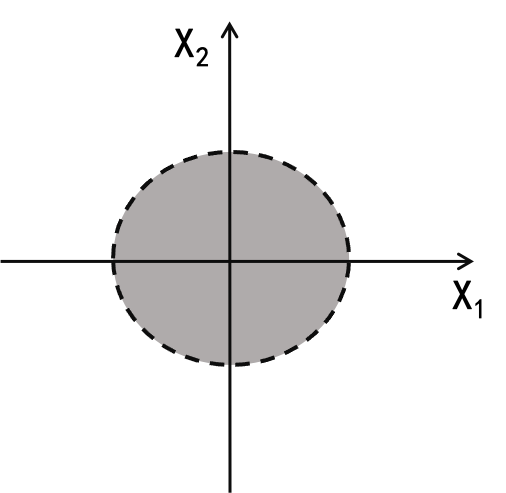
\includegraphics[width=0.28\textwidth]{figs/4.png}
      \end{center}
      \[ \Delta X_1 = \Delta X_2  = \frac{1}{2}\]
真空态的量子涨落为量子噪音的极限(极小值$\dfrac{1}{4}$) 
\end{frame}

\section{5. 相位算符}

\begin{frame} 
  \frametitle{相位算符的定义}
       经典光场的复振幅 
       \[ a= \left|a\right| e^{i\varphi}\]
       经典光场的正则分量
       \[ q(t) = a e^{-\omega t} + a e^{\omega t} = 2\left|a \right|\cos(\omega t + \varphi)\]
       (1) 那是否可写出一个相位算符呢?, 比如把湮灭算符写成
       \[ \hat{a} = \hat{g} e ^ {i \hat{\varphi}} \]
       这种写法是不行的, 因为
       $e ^ {i \hat{\varphi}}$与$e ^ {-i \hat{\varphi}}$ 并不是幺正的, 会导致 $\hat{\varphi}$不是厄密的,因而没有可测量意义. 
\end{frame}

\begin{frame} 
    \frametitle{}
    ~\\
       (2) 为保证厄密, Susskind–Glogower, 令
       \[ \rs{\varphi} = \sum_ {n=0} ^ \infty e^{i (n\varphi)} \rs{n} \]
       定义指数算符
       \[ \hat {e} \rs{\varphi}= e^{i {\varphi}}\rs{\varphi} \] 
        \[ \ls{\varphi}  e^{-i {\varphi}} = \ls{\varphi} \hat{e}^{\dagger}\]
      可得指数算符与产生湮灭算符的关系
      \[ \hat {e} = \frac{1}{\sqrt{\hat{n}+1}} \hat {a} =  \frac{1}{\sqrt{\hat {a}\hat {a}^{\dagger}}} \hat {a} \] 
      \[ \hat {e}^{\dagger} = \hat {a}^{\dagger} \frac{1}{\sqrt{\hat{n}+1}} = \hat {a}^{\dagger} \frac{1}{\sqrt{\hat {a}\hat {a}^{\dagger}}}  \] 
\end{frame}

\begin{frame} 
\frametitle{}
定义新的相位算符
\[\hat{C}= \frac{1}{2} (\hat {e} + \hat {e}^{\dagger})=\frac{1}{2}\left[ \frac{1}{\sqrt{\hat{n}+1}}a + a^{\dagger}  \frac{1}{\sqrt{\hat{n}+1}}\right]\]
\[\hat{S}= \frac{1}{2i} (\hat {e} - \hat {e}^{\dagger})=\frac{1}{2i}\left[ \frac{1}{\sqrt{\hat{n}+1}}a - a^{\dagger}  \frac{1}{\sqrt{\hat{n}+1}}\right]\]
       反向求得 
       \[\hat{a}= \sqrt{\hat{n}+1}(\hat{C}+i\hat{S})\]
       \[\hat{a}^{\dagger}= (\hat{C}-i\hat{S})\sqrt{\hat{n}+1}\]
\end{frame}

\begin{frame} 
\frametitle{}
    \例 [6. 试证明指数算符有如下性质]
    {\[ \hat {e} \rs{n} = \rs{n-1}, \qquad \hat {e}^{\dagger} \rs{n} = \rs{n+1}\]}
    \证 ~
    \[ \begin{aligned}
      \hat {e} \rs{n} & = \frac{1}{\sqrt{\hat{n}+1}} \hat {a} \rs{n}\\
      &= \frac{1}{\sqrt{\hat{n}+1}}  \sqrt{n} \rs{n-1} \\
      &= \frac{1}{\sqrt{(n-1)+1}}  \sqrt{n} \rs{n-1}  \\ 
      &= \rs{n-1}
    \end{aligned}\] 
\end{frame}

\begin{frame} 
\frametitle{相位算符的性质}
性质(1):
\[ \begin{aligned}
        S \rs{n} &= \frac{1}{2i} [\rs{n-1}+\rs{n-1}]\\
        S \rs{0} &=-\frac{1}{2i} \rs{1}\\
        S^2 \rs{n}&= \frac{1}{4} [\rs{n}+\rs{n}- \rs{n-2}-\rs{n+2}] \\  
     \end{aligned}\] 
\end{frame}

%\begin{frame} 
%\frametitle{}
%相干态的相位均值:
%    \[  \left\langle \alpha |C| \alpha   \right\rangle = %\left|\alpha\right|\cos\theta \exp(-\left|\alpha\right|%^2) \sum_n \frac{\left|\alpha\right|^{2n}}{n! \sqrt{n+1}%} \]
%    当 $\left|\alpha\right|^2\gg 1$时
%    \[  \left\langle \alpha |\cos \varphi| \alpha   %\right\rangle = \cos \theta (1+ \frac{1}{8\left|%\alpha\right|^2}+ \cdots )\]
%    \[  \left\langle \alpha |\sin \varphi| \alpha   %\right\rangle = \cos^2 \theta -\frac{\cos^2 \theta %-\frac{1}{2}}{2\left|\alpha\right|^2 } \]   
%\end{frame}

\begin{frame} 
\frametitle{}
性质(2):
\[ \begin{aligned}
        [C, S] & = \frac{1}{2}i \rl{0}{0}\\
        [C, \hat {n} ] & = i S \\ 
        [S, \hat {n} ] & = -i C \\ 
        C^2 + S^2 &= 1-\frac{1}{2} \rl{0}{0} 
     \end{aligned}\] 
(3) 数态的相位均值
   \[ \left\langle n|C|n \right\rangle = \left\langle n|S|n \right\rangle =0 \]
这正是光场电磁分量均值为零的原因
   \[ \left\langle n|C^2|n \right\rangle = \left\langle n|S^2|n \right\rangle = 
   \begin{cases}
    \frac{1}{2} \quad  n \ge 1 \\ 
    ~\\
    \frac{1}{4} \quad  n = 0
   \end{cases} \]
\end{frame}

\begin{frame} 
\frametitle{}
    \例 [7. 设光场处于数态叠加态, 求相位分布函数]{}
    \解 ~光场 
    \[ \rs{\psi} = \sum c_n \rs{n} \]
     方法(1) : \\
    相位表象的波函数
     \[ \lr{\varphi}{\psi} = \sum_ {n=0} ^ \infty e^{-i (n\varphi)} c_n \lr{n} {n} \]
     相位分布 
     \[ \begin{aligned}
       P(\varphi) &= \frac{1}{2 \pi} |\lr{\varphi}{\psi} |^2 \\
       &= \frac{1}{2 \pi} | \sum_ {n=0} ^ \infty e^{-i (n\varphi)} c_n  |^2 \\
     \end{aligned}\] 
     对于具体的叠加态, 可得分布函数
\end{frame}

\begin{frame} 
\frametitle{}
     方法(2) : \\
     密度算符
     \[ \rho = \rl{\psi}{\psi} \]
     相位分布
     \[ \begin{aligned}
      P(\varphi) &= \frac{1}{2 \pi} \lcr{\varphi}{\rho} {\varphi} \\
      &= \frac{1}{2 \pi} \lr{\varphi}{\psi} \lr{\psi}{\varphi} \\
      &= \cdots
    \end{aligned}\] 
     * 密度算符方法算混态更方便...
     \[ \rho = \sum_j P_j\rl{\psi_j}{\psi_j} \]
\end{frame}

\section{6. 自由光场的量子化}

\begin{frame}
      \frametitle{自由光场的单模量子化}
      自由空间电磁场为平面波(行波解):
      \[  \hat{e}_\sigma exp (\pm i (\omega_k t - \mathbf{k}\cdot \mathbf{r})), \qquad k^2 =\frac{\omega_k ^2}{c^2} \]
      式中 $\hat{e}_\sigma $ 为偏振方向上的单位矢量, $\sigma=\pm$ 代表两个振动方向, 它们相互正交且都与波矢$\mathbf{k}$正交. \\ \vspace*{1em} 
      经箱归一化, 可离散化行波, 得 
      \[ \mathbf{k} = \frac{2\pi}{L} (l_1 \mathbf{i} + l_2 \mathbf{j}+ l_3 \mathbf{k}), \qquad l_i= 0, \pm 1, \pm 2, \cdots \]
      行波本征模为
      \[ \mathbf{u}_{k\sigma} (\mathbf{r}) = \hat{e}_\sigma e^{i \mathbf{k}\cdot \mathbf{r}}\]
\end{frame} 

\begin{frame}
      \frametitle{}
    自由空间电磁场行波展开
      \[   \begin{aligned}
        \mathbf{E} (\mathbf{r},t) &=i \sum^\infty _{k,\sigma} (\frac{\hbar\omega_k}{2 \epsilon_0 V } )^{1/2} \hat{e}_\sigma [ a_{k\sigma} (t) e^{i \mathbf{k}\cdot \mathbf{r}} - a ^* _{k\sigma} (t)  e^{-i \mathbf{k}\cdot \mathbf{r}}] \\
      \mathbf{H} (\mathbf{r},t) &=i \sum^\infty _{k,\sigma} (\frac{\hbar\omega_k}{2 \mu_0 V } )^{1/2} (\hat{e}_k \times \hat{e}_\sigma) [ a_{k\sigma} (t) e^{i \mathbf{k}\cdot \mathbf{r}} - a ^* _{k\sigma} (t)  e^{-i \mathbf{k}\cdot \mathbf{r}}] 
      \end{aligned} \]
    箱内总能量:
      \[ \begin{aligned}
        H &= \frac{1}{2} \int_V (\mu_0 \mathbf{H}^2 + \epsilon_0 \mathbf{E}^2) dV \\ 
        &= \frac{1}{2}\sum^\infty _{k,\sigma} (p_{k\sigma} ^2 + \omega_k ^2 q_{k\sigma} ^2 )  \\ 
        & = \sum^\infty _{k,\sigma} H_{k\sigma}
      \end{aligned} 
      \] 
\end{frame}

\begin{frame}
      \frametitle{}
      单色行波的哈密顿
      \[ H_{k\sigma} = \frac{1}{2} (p_{k\sigma} ^2 + \omega_k ^2 q_{k\sigma} ^2)\]
      哈密顿运动方程
        \[ \begin{aligned}
        \frac{\mathrm{d}p_{k\sigma}}{\mathrm{d}t} &= - \frac{\partial H_{k\sigma}}{\partial q_{k\sigma}} = - \omega ^2 _{k\sigma} q_{k\sigma} \\ 
        \frac{\mathrm{d}q_{k\sigma}}{\mathrm{d}t} &= \frac{\partial H_{k\sigma}}{\partial p_{k\sigma}} =p_{k\sigma}
        \end{aligned} 
      \] 
\end{frame}

\begin{frame}        
      同理,正则量子化
      \[ \hat{H}_{k\sigma} = \frac{1}{2} (\hat{p}_{k\sigma} ^2 + \omega_k ^2 \hat{q}_{k\sigma} ^2) \qquad \text{with} \quad [\hat{p}_{k\sigma},\hat{q}_{k\sigma}] =i\hbar \]

      \[ \hat{H}_{k\sigma}= \hbar \omega_{k\sigma} \left(\hat{a}^\dagger _{k\sigma} \hat{a} _{k\sigma}+ \frac{1 }{2}\right) \qquad \text{with} \quad [\hat{a} _{k\sigma},\hat{a}^\dagger _{k\sigma}]=1 \]
      行波电场和磁场算符:
      \[ \begin{cases}
        \hat{\mathbf{E}} (\mathbf{r},t)&=i \sum^\infty _{k,\sigma} (\frac{\hbar\omega_k}{2 \epsilon_0 V } )^{1/2} \hat{e}_\sigma [ \hat{a} _{k\sigma} (t) e^{i \mathbf{k}\cdot \mathbf{r}} - \hat{a} ^\dagger _{k\sigma} (t)  e^{-i \mathbf{k}\cdot \mathbf{r}}] \\
        &= \hat{\mathbf{E}}^+(\mathbf{r},t)+ \hat{\mathbf{E}}^-(\mathbf{r},t) \\
        ~\\
      \hat{\mathbf{H}} (\mathbf{r},t) &=i \sum^\infty _{k,\sigma} (\frac{\hbar\omega_k}{2 \mu_0 V } )^{1/2} (\hat{e}_k \times \hat{e}_\sigma) [ \hat{a} _{k\sigma} (t) e^{i \mathbf{k}\cdot \mathbf{r}} - \hat{a} ^\dagger _{k\sigma} (t)  e^{-i \mathbf{k}\cdot \mathbf{r}}] 
      \end{cases} \]
\end{frame}

\begin{frame}
  \frametitle{}
  \例[8.考虑单模行波场, 求电场和磁场强度的量子涨落]{}
  \解~ 单模行波场的电场为
  \[ \mathbf{E}_l(\mathbf{r},t) = E_{0} (\hat{a}_l\exp^{-i \omega t + i \mathbf{k}\cdot \mathbf{r}} + \hat{a}_l ^\dagger \exp^{i \omega t - i \mathbf{k}\cdot \mathbf{r}})\]
  设光场处于$Fock$态$\rs{n}$, 电场的平均值: 
\[ 
\begin{aligned}
        \left\langle \mathbf{E}_l(\mathbf{r},t) \right\rangle &=\lcr{n}{\mathbf{E}_l(\mathbf{r},t)}{n} \\  
        &= \lcr{n}{E_{0} (\hat{a}_l \exp^{-i \omega t + i \mathbf{k}\cdot \mathbf{r}} +\hat{a}_l ^\dagger \exp^{i \omega t - i \mathbf{k}\cdot \mathbf{r}})}{n}\\ 
        &=0 
\end{aligned}\]
\end{frame}

\begin{frame}
  \frametitle{}
  \[ \begin{aligned}
    \left\langle \mathbf{E}^2_l(\mathbf{r},t) \right\rangle &=\lcr{n}{\mathbf{E}^2_l(\mathbf{r},t)}{n} \\  
    &= E^2_{0} \lcr{n}{(\hat{a}_l \exp^{-i \omega t + i \mathbf{k}\cdot \mathbf{r}} +\hat{a}_l ^\dagger \exp^{i \omega t - i \mathbf{k}\cdot \mathbf{r}})^2}{n}\\ 
    &= E^2_{0} \lcr{n}{\hat{a}_l\hat{a}_l ^\dagger + \hat{a}_l ^\dagger \hat{a}_l}{n}\\ 
    &= E^2_{0} \lcr{n}{\sqrt{(n+1)(n+1)} + \sqrt{nn}}{n}\\ 
    &= E^2_{0} (2n+1)
\end{aligned}\]
量子涨落: 
\[
\begin{aligned}
    \Delta \mathbf{E}_l &= \sqrt{\langle \mathbf{E}^2 _l \rangle - \langle \mathbf{E}_l \rangle ^2} \\
    &= E_0 \sqrt{2n+1}
\end{aligned} \]
即使没有激发(n=0),依然存在真空涨落$ E_0 $  
\end{frame}

\begin{frame} 
\frametitle{多模光场的量子化}
  能量是对所有模求和
   \[ \hat{H} = \sum_l \hbar \omega_l (\hat{n}_l + \frac{1}{2}) = \sum_l \frac{1}{2} \hbar \omega_l(a^{\dagger}_l a_l + a_la^{\dagger}_l ) \]
   能量本征态是各模数态的张量积
   \[ \rs{\{n_l\}}=\rs{n_1}\otimes \rs{n_2}\otimes \rs{n_3}\cdots\rs{n_l}\cdots = \rs{n_1, n_2, n_3, \cdots, n_l,\cdots }\]
  能量本征方程
  \[ \hat{H} \rs{\{n_l\}} = E \rs{\{n_l\}}\]
  根据张量空间运算法则
  \[ \hat{a}_l \rs{\{n_l\}} = \sqrt{n_l} \rs{n_1, n_2, n_3, \cdots, n_l-1,\cdots }\]
  \[  \ls{n_1, n_2, n_3, \cdots, n_l+1,\cdots }\sqrt{n_l+1}=  \ls{\{n_l\}}\hat{a}^{\dagger}_l \]
\end{frame}

\begin{frame} 
  \frametitle{}
  \例[9. 计算双模场算符Q的均值]{
    \[  Q= \Omega \sum_{i,j,k,l} a^{\dagger} _i a^{\dagger} _j a_k a_l, \qquad i,j,k,l =1,2 \]}
    \解 双模应对双光子态进行计算
    \[ \begin{aligned}
        \overline{Q}&= \left\langle n_1 n_2|Q|n_2n_1  \right\rangle \\
        &= \Omega[\left\langle n_1 n_2|a^{\dagger} _1 a^{\dagger} _1 a_1 a_1|n_2n_1  \right\rangle + \left\langle n_1 n_2|a^{\dagger} _1 a^{\dagger} _2 a_1 a_2|n_2n_1  \right\rangle \\ 
        & + \left\langle n_1 n_2|a^{\dagger} _1 a^{\dagger} _2 a_1 a_2|n_2n_1  \right\rangle  
        + \left\langle n_1 n_2|a^{\dagger} _2 a^{\dagger} _2 a_2 a_2|n_2n_1  \right\rangle]  \\
        &= \Omega [(n_1 ^2 -n_1) + (n_2 ^2 -n_2) +4n_1 n_2 ]
    \end{aligned}\]    
 \end{frame}

 \begin{frame} 
 \frametitle{}
     * 计算第一项 
  \[ \begin{aligned}
  \left\langle n_1 n_2|a^{\dagger} _1 a^{\dagger} _1 a_1 a_1|n_2n_1  \right\rangle  &= \left\langle n_1|a^{\dagger} _1 a^{\dagger} _1 a_1 a_1|n_1  \right\rangle \\ 
  &= \left\langle n_1|a^{\dagger} _1 (a_1a^{\dagger} _1 -1) a_1|n_1  \right\rangle \\ 
  &= \left\langle n_1|(a^{\dagger} _1 a_1a^{\dagger} a_1 - a^{\dagger} a_1) |n_1  \right\rangle \\ 
  &= \left\langle n_1|(a^{\dagger} _1 a_1)^2 |n_1 \right\rangle - \left\langle n_1| a^{\dagger} a_1 |n_1  \right\rangle\\ 
  &= \left\langle n_1|\hat{n}^2 _1 |n_1 \right\rangle - \left\langle n_1| \hat{n}_1 |n_1  \right\rangle\\ 
  &= n_1 ^2 -n_1
 \end{aligned}\]
 * 课堂作业: 计算第二项
\end{frame}

\begin{frame} 
  \frametitle{小结:}
    (1) 光场哈密顿可分解为一系列场谐振子哈密顿
    \[ \hat{H}_{k\sigma}= \sum_{k,\sigma}\hbar \omega_{k\sigma} \left(\hat{a}^\dagger _{k\sigma} \hat{a} _{k\sigma}+ \frac{1 }{2}\right) \qquad \text{with} \quad [\hat{a} _{k\sigma},\hat{a}^\dagger _{k\sigma}]=1 \]
    (2) 自由光场可表示为一系列量子化的平面波 
    \[\begin{aligned}
      \hat{\mathbf{E}} (\mathbf{r},t) &=i \sum^\infty _{k,\sigma} (\frac{\hbar\omega_k}{2 \epsilon_0 V } )^{1/2} \hat{e}_\sigma \left[ \hat{a} _{k\sigma} (t) e^{i \mathbf{k}\cdot \mathbf{r}} - \hat{a} ^\dagger _{k\sigma} (t)  e^{-i \mathbf{k}\cdot \mathbf{r}}\right] \\
      &= \hat{\mathbf{E}}^+(\mathbf{r},t)+ \hat{\mathbf{E}}^-(\mathbf{r},t)
    \end{aligned} \]
    (3) 腔场则可表示为一系列量子化的驻波
  \end{frame}

%%%%%%%%%%%%%%%%%%%%%%%%%%%%%%%%%%%%%%%%%%%%%%%%%%%%%%%%%%%%%%%%%%%
\begin{frame}
    \frametitle{课外作业}
    \begin{enumerate}
        \item  利用腔模正交性证明 \[ H= \sum_l H_l\]
        \item  计算电磁场真空态的量子涨落
        \item  试证明,只有光场处于两相临数态的叠加态时,电场算符的均值才不为零
        \item  已知光场处于如下混态, 求相位分布  \[ \rho = \frac{1}{2}(\rl{0}{0} + \rl{1}{1} ) \]
    \end{enumerate}
\end{frame}
%%%%%%%%%%%%%%%%%%%%%%%%%%%%%%%%%%%%%%%%%%%%%%%%%%%%%%%%%%%%%%%%%%%